%!TEX root = ../main.tex
%
\section{Ball and plate}
\begin{frame}
	\frametitle{Ball and plate}
\end{frame}
%
\begin{frame}
\frametitle{Ball and plate}
%
\begin{figure}
		{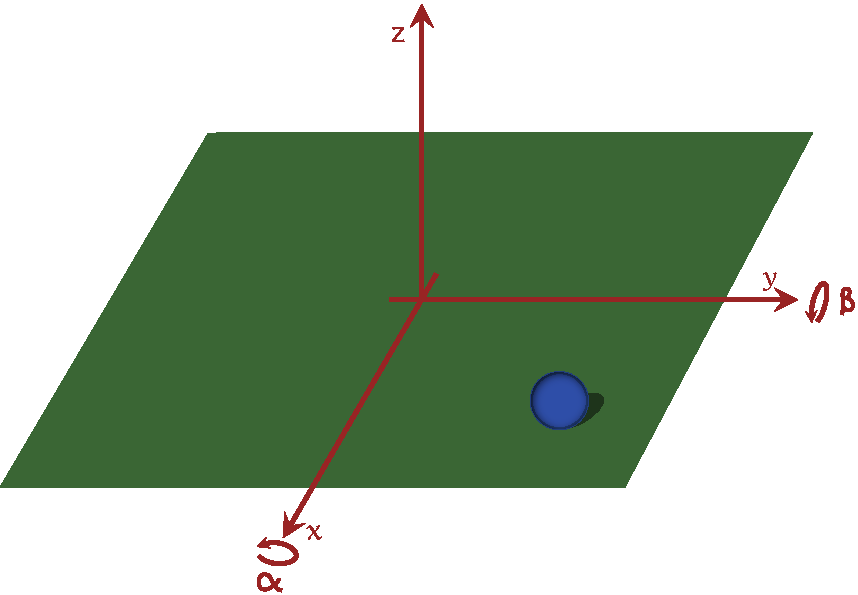
\includegraphics[width=.8\linewidth]{img/ballplate.pdf}}
		\caption{Coordinate frame of the ball and plate system}
		\label{fig:BallPlate}
\end{figure}
\end{frame}
%
\begin{frame}
\frametitle{Ball and plate - Parameters}
\begin{table}
\begin{center}
\begin{tabu} to \textwidth { | X[c] | X[c] | X[c] | }
	\hline
	\textbf{Parameter} & \textbf{Description} & \textbf{Value} \\
	\hline
	$m$ & Mass of the ball & $0.0109 \, Kg$ \\
	$r$ & Radius of the ball & $0.01 \, m$ \\
	$I_b$ & Ball inertia & $4.3563e^{-7} \, Kg\times m^2$ \\
	$l_p$ & Plate side & $0.6 \, m$ \\
	$I_p$ & Plate inertia & $0.175 \, Kg\times m^2$ \\
	\hline
\end{tabu}
\caption{Ball and plate geometric and dynamic parameters}
\label{tab:BallPlate_param}
\end{center}
\end{table}
\end{frame}
%
\subsection{Dynamic}
\begin{frame}
\frametitle{Ball and plate - Dynamic model}
%
The general form of Euler-Lagrange for dynamic equations is used to describe the system:
%
\begin{equation}
	\frac{d}{dt}\frac{\delta T}{\delta q_i} - \frac{\delta T}{\delta q_i} + \frac{\delta V}{\delta q_i} = Q_i
\end{equation}
%
Where $T$ is the kinetic energy, $V$ is the potential energy, $Q_i$ is the i-th generalized force and $q_i$ id the i-th generalized coordinate. As generalized force we consider two torques acting on the plate $(Q_\alpha = \tau_\alpha, Q_\beta = \tau_\beta)$. As generalized coordinates we select two ball position coordinates $[x, y]$ on the frame fixed to the plate and two plate inclination $[\alpha, \beta]$.
\end{frame}
%
\begin{frame}
\frametitle{Ball and plate - Dynamic model}
%
Kinetic energy of the ball:
\begin{equation}
	T_{b} = \frac{1}{2}mv^2 + \frac{1}{2}I_b\omega^2 = \frac{1}{2}\left(m+\frac{I_b}{r^2}\right)\left(\dot{x}^2+\dot{y}^2\right)
\end{equation}
%
Kinetic energy of the plate:
\begin{equation}
	T_{p} = \frac{1}{2}\left(I_b + I_p\right)\left(\dot{\alpha} + \dot{\beta}\right) + \frac{1}{2}m\left(\dot{\alpha}x + \dot{\beta}y\right)^2
\end{equation}
%
Potential energy:
\begin{equation}
	V = mgh = mg(x\,sin\alpha + y\,sin\beta)
\end{equation}
\end{frame}
%
\begin{frame}
\frametitle{Ball and plate - Dynamic model}
%
After some derivations we find the following non-linear system of equations:
%
\begin{align}
	\left(m + \frac{I_b}{r^2}\right)\ddot{x} &- m\left(\dot{\alpha}\dot{\beta}y + \dot{\alpha}^2x\right)+mg\,sin\alpha = 0 \nonumber \\
	\left(m + \frac{I_b}{r^2}\right)\ddot{y} &- m\left(\dot{\alpha}\dot{\beta}x + \dot{\beta}^2y\right)+mg\,sin\beta = 0 \\
	\left(I_p + I_b + mx^2\right)\ddot{\alpha} &+ m\left(\ddot{\beta}xy + \dot{\beta}\left(\dot{x}y + x\dot{y}\right) + 2\dot{\alpha}\dot{x}x\right) +mgx\,cos{\alpha} = \tau_\alpha \nonumber \\
	\left(I_p + I_b + my^2\right)\ddot{\beta} &+ m\left(\ddot{\alpha}xy + \dot{\alpha}\left(\dot{x}y + x\dot{y}\right) + 2\dot{\beta}\dot{y}y\right) +mgy\,cos{\beta} = \tau_\beta \nonumber
\end{align}
\end{frame}
%
\begin{frame}
\frametitle{Ball and plate - Dynamic model}
%
We express the dynamic in matrix form:
%
\begin{equation}
\begin{aligned}
M(q) &=%
\begin{pmatrix}
	\left(m + \frac{I_b}{r^2}\right) &0 &0 &0\\
	0 &\left(m + \frac{I_b}{r^2}\right) &0 &0\\
	0 &0 &\left(I_b + I_p + mx^2\right) &mxy\\
	0 &0 &mxy &\left(I_b + I_p + my^2\right)
\end{pmatrix}\\
C(q,\dot{q}) &=%
\begin{pmatrix}
	0 &0 &-\dot{\alpha} x &-\dot{\alpha} y\\
	0 &0 &-\dot{\beta} x &-\dot{\beta} y\\
	2\dot{\alpha}x &0 &0 &\left(\dot{x}y+x\dot{y}\right)\\
	0 &2\dot{\beta}y &\left(\dot{x}y+x\dot{y}\right) &0
\end{pmatrix}\\
G(q) &=%
\begin{pmatrix}
	mg\,sin\alpha\\
	mg\,sin\beta\\
	mgx\,cos\alpha\\
	mgx\,cos\beta
\end{pmatrix}
\end{aligned}
\end{equation}
\end{frame}
%
\begin{frame}
\frametitle{Ball and plate - Dynamic model}
%
\textbf{Affine-in-control formulation}:
\begin{equation}
	\dot{x} =%
	\begin{pmatrix}
	x_5\\ x_6\\ x_7\\ x_8\\ -B(q)^{-1}\left(C(q,\dot{q})\dot{q}+G(q)\right)
	\end{pmatrix}
	+
	\begin{pmatrix}
		0_{4\times2}\\
		B(q)^{-1}
	\end{pmatrix}
	\begin{pmatrix}
		\tau_1\\
	 	\tau_2
	\end{pmatrix}
\end{equation}
Where
\[x = (x_b, y_b, \alpha, \beta, \dot{x_b}, \dot{y_b}, \dot{\alpha}, \dot{\beta})^T\]
\end{frame}
%
\begin{frame}
\frametitle{Ball and plate - Dynamic model}
\textbf{Change of coordinates}:
\begin{align}
	u_1 = 2mx\dot{x}\dot{\alpha} - mgx\,cos\alpha - \left(I_p + I_b + mx^2\right)\ddot{\alpha} - m\dot{\beta}\left(\dot{x}y + \dot{y}x\right) - 2m\dot{\alpha}\dot{x}x \nonumber \\
	u_2 = 2my\dot{y}\dot{\beta} - mgy\,cos\beta - \left(I_p + I_b + my^2\right)\ddot{\beta} - m\dot{\alpha}\left(\dot{x}y + \dot{y}x\right) - 2m\dot{\beta}\dot{y}y \nonumber \\
\end{align}
\end{frame}
%
\subsection{Structural properties}
\subsubsection{Controllability}
\begin{frame}
\frametitle{Controllability}
Chow theorem.
\end{frame}
\begin{frame}
\frametitle{Controllability}
\begin{equation}
	Q(x) =%
	\begin{pmatrix}
		0 &0  &\star &\star &\star &\star &\star &\star &0 &0 &0 &0 &0 &0 &0 &0 \\
		0 &0  &0 &0 &0 &0 &0 &0 &0 &0 &\star &\star &\star &\star &\star &\star \\
		0 &-1 &0 &0 &0 &0 &0 &0 &0 &0 &0 &0 &0 &0 &0 &0 \\
		0 &0  &0 &0 &0 &0 &0 &0 &0 &-1 &0 &0 &0 &0 &0 &0 \\
		0 &\star &\star &\star &\star &\star &\star &\star &0 &0 &0 &0 &0 &0 &0 &0 \\
		0 &0  &0 &0 &0 &0 &0 &0 &0 &\star &\star &\star &\star &\star &\star &\star \\
		1 &0  &0 &0 &0 &0 &0 &0 &0 &0 &0 &0 &0 &0 &0 &0 \\
		0 &0  &0 &0 &0 &0 &0 &0 &1 &0 &0 &0 &0 &0 &0 &0
	\end{pmatrix}
\end{equation}\\[10pt]
Where the $\star$ elements represent the non constant terms of the $Q$ matrix.
\end{frame}
%
\begin{frame}
\frametitle{Controllability}
Performing row swapping, in order to calculate the matrix rank, we obtain the matrix
$\tilde{Q}(x)$ as follows:\\[10pt]
\begin{equation}
	\tilde{Q}(x)=%
	\begin{pmatrix}
		1 &0     &0     &0     &0     &0     &0     &0 &\dots \\
		0 &\star &\star &0     &\star &0     &0     &0 &\dots \\
		0 &\star &\star &0     &0     &0     &0     &0 &\dots \\
		0 &0     &0     &\star &0     &0     &\star &0 &\dots \\
		0 &0     &0     &0     &-1    &0     &0     &0 &\dots \\
		0 &0     &0     &0     &0     &-1    &0     &0 &\dots \\
		0 &0     &0     &\star &0     &\star &\star &0 &\dots \\
		0 &0     &0     &0     &0     &0     &0     &1 &\dots
	\end{pmatrix}_{8\times16}
\end{equation}
\end{frame}
%
\begin{frame}
\frametitle{Controllability}
\textbf{Rank condition.} Evaluating the rank of matrix $\tilde{Q}(x_0)$ in the equilibria, the following cases are obtained:
\begin{itemize}
	\item $x_4 \equiv \pi/2,\; x_8 \equiv 0\; \implies rank(Q(x_0))<8$.\\ Which represent the physical condition where $\beta = \pi/2$ with null angular velocity, the system is out of the range of interest.
	\item $x_3 \equiv \pi/2,\; x_7 \equiv 0\; \implies rank(Q(x_0))<8$.\\ Which represent the physical condition where $\alpha = \pi/2$ with null angular velocity; the same arguments as above hold.
	\item In all other cases we find $rank(Q(x_0))=8$ and the rank condition of controllability is satisfied.
\end{itemize}
\end{frame}
%
\subsubsection{Observability}
\begin{frame}
\frametitle{Observability}
\end{frame}
%
\subsection{Feedback linearization}
\begin{frame}
\frametitle{Approximated Feedback linearization}
\end{frame}
%
\subsection{Control}
\begin{frame}
\frametitle{PID Control}
\end{frame}